\documentclass[border=0mm]{standalone}
\usepackage{pgfplots}
\usepgfplotslibrary{groupplots}
\pgfplotsset{compat=1.17}
\usepackage{xcolor}

\definecolor{color1}{rgb}{0,0.4470,0.7410}
\definecolor{color2}{rgb}{0.8500,0.3250,0.0980}
\definecolor{color3}{rgb}{0.9290,0.6940,0.1250}
\definecolor{color4}{rgb}{0.4940,0.1840,0.5560}
\definecolor{color5}{rgb}{0.4660,0.6740,0.1880}

\definecolor{lightblue}{RGB}{86,192,150}  % Define light blue color





\pgfdeclarelayer{background layer}%
\pgfdeclarelayer{foreground layer}%
\pgfsetlayers{background layer,main,foreground layer}%
\begin{document}
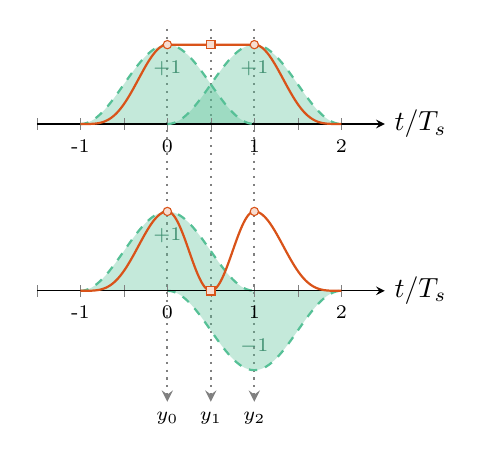
\begin{tikzpicture}
\begin{groupplot}[
group style={
    group name=my plots,
    group size= 1 by 2,  % 1 row and 2 columns
    horizontal sep=1.5cm,  % Adjust horizontal separation between subplots
    vertical sep=-0.3cm,  % Adjust horizontal separation between subplots
  },
  width = 6cm,
  height = 4cm,
  xlabel={$t/T_s$},
  axis x line=middle,  % Show only the x-axis
  axis y line=none,    % Hide the y-axis
  xmin=-1.5, xmax=2.5,
  ymin=-0.6, ymax=0.6,  % Set ymax to 2
  xtick={-2,-1.5,...,2},
  xticklabels={-2,,-1,,0,,1,,2},
  tick label style={font=\scriptsize},
  xlabel style={
    right,
  },
]%

\nextgroupplot
\begin{pgfonlayer}{background layer}
\addplot[lightblue, domain=-1:1, samples=100, draw=none, fill=lightblue, fill opacity=0.35] {0.25*(1+cos(deg(pi*x)))};
\addplot[lightblue, domain=0:2, samples=100, draw=none, fill=lightblue, fill opacity=0.35] {0.25*(1+cos(deg(pi*(x-1))))};
\end{pgfonlayer}

\addplot[lightblue, domain=-1:1, samples=100, dashed, thick] {0.25*(1+cos(deg(pi*x)))};
\addplot[lightblue, domain=0:2, samples=100, dashed, thick] {0.25*(1+cos(deg(pi*(x-1))))};


\addplot[color2, domain=-1:0, samples=100, thick] {2*(0.25*(1+cos(deg(pi*x))))^2};
\addplot[color2, domain=0:1, samples=100, thick] {2*(0.25*(1+cos(deg(pi*x)))+0.25*(1+cos(deg(pi*(x-1)))))^2};
\addplot[color2, domain=1:2, samples=100, thick] {2*(0.25*(1+cos(deg(pi*(x-1)))))^2};
\addplot[only marks, mark=*, mark size=1.5pt, mark options={draw=color2, fill=color2!20}] coordinates{(0,0.5)(1, 0.5)};
\addplot[only marks, mark=square*, mark size=1.5pt, mark options={draw=color2, fill=color2!20}] coordinates{(0.5, 0.5)};

\coordinate (p3) at (axis cs: 0,0.35);
\coordinate (p4) at (axis cs: 1,0.35);
\coordinate (top21) at (axis cs:0,\pgfkeysvalueof{/pgfplots/ymax});
\coordinate (top22) at (axis cs:0.5,\pgfkeysvalueof{/pgfplots/ymax});
\coordinate (top23) at (axis cs:1,\pgfkeysvalueof{/pgfplots/ymax});

\nextgroupplot
\begin{pgfonlayer}{background layer}
\addplot[lightblue, domain=-1:1, samples=100, dashed, thick, fill=lightblue, fill opacity=0.35] {0.25*(1+cos(deg(pi*x)))};
\addplot[lightblue, domain=0:2, samples=100, dashed, thick, fill=lightblue, fill opacity=0.35] {-0.25*(1+cos(deg(pi*(x-1))))};
\end{pgfonlayer}

\addplot[color2, domain=-1:0, samples=100, thick] {2*(0.25*(1+cos(deg(pi*x))))^2};
\addplot[color2, domain=0:1, samples=100, thick] {2*(0.25*(1+cos(deg(pi*x)))-0.25*(1+cos(deg(pi*(x-1)))))^2};
\addplot[color2, domain=1:2, samples=100, thick] {2*(0.25*(1+cos(deg(pi*(x-1)))))^2};
\addplot[only marks, mark=*, mark size=1.5pt, mark options={draw=color2, fill=color2!20}] coordinates{(0,0.5)(1, 0.5)};
\addplot[only marks, mark=square*, mark size=1.5pt, mark options={draw=color2, fill=color2!20}] coordinates{(0.5, 0)};

\coordinate (p7) at (axis cs: 0,0.35);
\coordinate (p8) at (axis cs: 1,-0.35);
\coordinate (bot21) at (axis cs:0,\pgfkeysvalueof{/pgfplots/ymin});
\coordinate (bot22) at (axis cs:0.5,\pgfkeysvalueof{/pgfplots/ymin});
\coordinate (bot23) at (axis cs:1,\pgfkeysvalueof{/pgfplots/ymin});


\end{groupplot}

\begin{pgfonlayer}{background layer}
\draw [thick, dotted,-stealth, black!50] (top21) -- (bot21) --+ (0,-0.2) node [below, black, font=\scriptsize] {$y_0$};
\draw [thick, dotted,-stealth, black!50] (top22) -- (bot22) --+ (0,-0.2) node [below, black, font=\scriptsize] {$y_1$};
\draw [thick, dotted,-stealth, black!50] (top23) -- (bot23) --+ (0,-0.2) node [below, black, font=\scriptsize] {$y_2$};
\end{pgfonlayer}

\node  at (p3) [font=\scriptsize, text=lightblue!75!black]{$+1$};
\node  at (p4) [font=\scriptsize, text=lightblue!75!black]{$+1$};
\node  at (p7) [font=\scriptsize, text=lightblue!75!black]{$+1$};
\node  at (p8) [font=\scriptsize, text=lightblue!75!black]{$-1$};


\end{tikzpicture}

\end{document}
























